%DESIGN OVERVIEW
\subsection{Steganography and CovertFS}
% Section needs additional research
The primary purpose in a web based covert file system is confidentiality and plausible deniability. Using steganography can provide both confidentiality for users as well as plausible deniability. However, steganography has risks that make it vulnerable to both. Statistical analysis and visible alterations (anything else? -- research) can make steganography detectable, thus removing the aspect of both confidentiality and plausible deniability. However, there are ways to reduce the risks of using steganography. 

\subsubsection{Risks Using Steganography}
%Not enough data
The greatest risk to using steganography, particularly our steganography module, is that an embedded message can be discovered using statistical analysis. Since the original images exist on Tumblr and can be retrieved using the Cat API, our images that get uploaded to Sendspace can be compared to the originals. Statistical analysis between the original and the modified images will indicate that a message has been embeded. There are alternative steganograhpy techniques, but their are still several steganalysis tools to detect them (cite http://www.computing.surrey.ac.uk/personal/st/H.Schaathun/projects/Past/leivaditis.pdf). Not only can steganalysis detected changes, but they are visually apparent as well. Figure A shows both an original image and an encoded image.
\caption{Figure A}
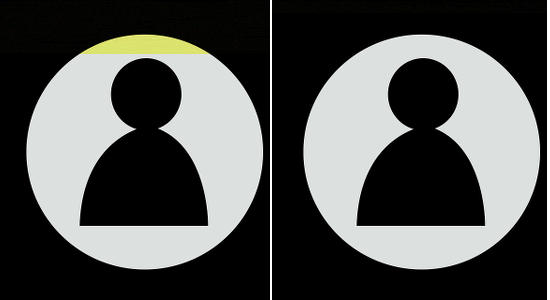
\includegraphics{comparison}
\subsubsection{}
The image on the left is the one with a message encoded into it. The image on the right is the original. Notice the yellow in the image on the left - that is the encoded message. Because the message was encoded into white pixels, the pixels' value changes noticably.  
Sometimes, the differences 
statistical analysis
		the original images exist online since we are using the Cat API
		perform statistical analysis
	many kinds of LSB can changes colors that the eye can bit up
	alternative steg techniques

\subsubsection{Mitigating Risks of Steganography}
%Not enough data
These risks are mitigated by the fact that there is no universal standard for steganography methods. A user can easily replace the steganography module that we offer with a module of their own. That way, even if someone knows an image is not the original, that person will still not know who encoded it, or what kind of module was using for the encoding.Also, an encryption module can easily be added to our application and used to encrypt messages before they are encoded into an image. So even if someone knows what kind of steganography module is being used to encode messages into images, that person will also have the added challenge of decrypting the information. Although, there is no research to indicate that encryption helps in fooling steganalysis tools. Finally, since the original images exist on the internet, it will limit the plausible deniability of the user. It can be called into question as to why a certain user is uploading images that do not belong to that user to an online image database. 
There is no universal standard for steg methods
		so even if someone knows an image is not the original, they don't really know who encoded it our how due to modularity of CovertFS
	Can use encryption
		can help with stat analysis (research)
Using original images instead of Cat API images, but this will lead to originals existing somewhere which can decrease plausible deniability 

%IMPLEMENTATION SECTION
\subsection{Encoding a File System}

The covert file system uses a drop in steganography module that takes in a bytearray object and returns a URL to an image. We used "least significant bit" steganography for this application because of its simplicity and reliability.

\subsubsection{Steganography Implementation}

Least significant bit (LSB) steganography is a Substitution type of steganography~\cite{Nosrati2011} that replaces the least significant bits in the image's pixels. Our steganography module is not true LSB steganography because we replace multiple bits in each pixel allowing us to encode one byte of data into every pixel. First, we break every byte of the message into three segments. Two segments of the byte will contain three bits, and one segment will contain two bits. Next, we replace the three least significant bits of the red component with the first three bit segment. The green component follows with replacing its least significant bits with the second three bit segment. Lastly, we replace the two least significant bits of the blue component with the remaining two bit segment of data. 

There are obvious drawbacks to our implementation of LSB steganography, primarily that the image may appear distorted as seen in Figure X and CovertFS images are X percent easier to detect using standard statistical analysis techniques as seen in figure X. However, this implementation enables us to store more bytes than other implementations of LSB steganography (CITATION OR EVIDENCE NEEDED) which decreases the latency in uploading and downloading images in large file systems.
 
\subsubsection{File System to Images}

The first step in encoding a file system is retrieving an image. We use "The Cat API" which retrieves a random cat picture from Tumblr(c). Once we retrieve the image we determine the number of bytes we can encode in the image by multiplying the height and width of the image, in pixels. Since we encode one byte per pixel, the result of height times width results in the total number of bytes of data we can encode in the image. Next, we take the data we are going to encode and append a special end of file encoding. Then, we break the data into two sets, the total bytes we can encode in the image we retrieved, and the rest of the data. Next, we encode the data into the image and upload the data, upload, append the URL and EOF, and repeat. 
%If the total length of the data is less than the amount of data the image can hold, we encode the data into the image using the steganography method and return the url to the hosted image. 


%Otherwise, we encode the most data we can recursively until all the data is encoded and we return the URL of the last image recorded. We do this by encoding  break the data into multiple segments. In this situation, we must prepare the data by splitting the data into the maximum data we can store and the rest of the data. We then encode the data 